\subsection{Definition of Process}

% definition
Policy says what action is allowed or required
Process is a sequence of tasks, with each task invoking policy enforcement 


A \gls{process} is a task broken into a specified set of subtask dependencies, typically with subtasks in a sequence. 
Each task is associated with the application of policies enforced by bureaucrats. 
% Also known as a procedure. 
Two distinguishing features in the context of bureaucracy are authorization and justification.  
A process has inputs and outputs. 
A process can be decomposed into other processes. 
Processes operate on both information and tangible objects. 
Processes require \href{https://en.wikipedia.org/wiki/Work_(physics)}{work} and time. 
Processes are carried out by people or machines.

% process and roles
processes depend on roles that have responsibility/authority
When there aren't sufficient staffing, then individuals wear multiple hats
Commonly leads to conflict of interest among roles, which is defeated by one person in multiple roles
eg "review the implementation" and "implement"

\href{https://en.wikipedia.org/wiki/Responsibility_assignment_matrix}{Responsibility Assignment Matrix}

% how does understanding process help me?
The point to understanding process and policy is so that you know when to work within versus work around, when to accept versus change, when to ignore, how to leverage, and how to design


\subsection{Why do processes exist?}


\subsubsection{Processes ensure consistent application of policy}

Processes are in response to
* allocate scarce resources
   * limit bad behavior; guardrails to prevent harm
   * addressing risk
       * justification is necessary. 
   * keep stakeholders informed

    
Without oversight processes, \href{https://en.wikipedia.org/wiki/Tragedy_of_the_commons}{tragedy of commons} occurs and malicious actors dominate.

\href{https://en.wikipedia.org/wiki/Tragedy_of_the_commons}{Tragedy of the Commons} says that when there is a shared resource, someone will try to get away with behavior that is harmful to the organization.

Create processes for oversight/review/approval
Each process may be justifiable, but the aggregate can feel unreasonably burdensome to subjects and bureaucrats.






\subsubsection{Processes exist to Simplify}
Compared to an ad hoc approach, processes are intended to simplify what could otherwise be complicated moral decisions, coordination challenges, or financial assessments. %The simplification benefits the bureaucrat's workload; rarely are benefits to the subjects of the bureaucracy.  



A positive view is that specialization allows narrow focus and thus deeper understanding and skill. An alternative perspective is that specialization allows for dumbing down the role, thus enabling a cheaper workforce. In that view process allows dumb individuals to, as a group accomplish complicated things.  As a specific example, consider the process of designing and building a car. That complexity is feasible to undertake for a skilled and knowledgeable individual, but the cheaper approach is to hire individuals capable of installing the passenger-side doors in an assembly line.

Process development is driving by Complexity.

\subsubsection{Processes exist for Scaling Throughput}

Processes improve scalability. Cite the pin factory example

Ford factory throughput comparison

\subsubsection{Processes decrease reliance on Social Relations}

For a given complexity and given scale, there are people who are more social and less social and therefore desire more or less process

there are people who want process and documentation and are confused as to how things are operating when those aren't present


social influence does not have visibility/transparency
In contrast, processes are easier to understand and to track

social influence is not antithetical to processes. There's always a mixture of the two


\subsubsection{Processes help new people}

New people are likely to arrive and ask what are the processes and where is the documentation?

People have been on a team for a long time say don't burden me with processes I just need to get things done using the relationships with the people I have.

In addition to not having formed a social network, there's a second reason new people seek processes.

Recently graduated people from school are used to the existence of formal processes at high school or university level. Therefore when they join a job, they expect a similar set of conditions for processes to exist and follow

\subsubsection{Processes exist as artifacts for Promotion}

Processes can arise organically (bottom up) or be created top-down




% dangers of process
The simplification and the neglect of specific circumstances results in process friction. Process friction manifest in practical waste, temporal and efficiency, emotional frustration, and social distrust of institutions.




\begin{figure}
    \centering
    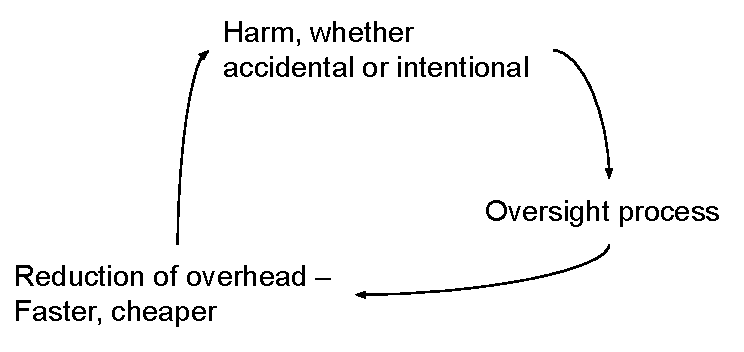
\includegraphics{images/process_loop_harm-oversight-improvement}
    \caption{loop: harm-oversight-improvement}
    \label{fig:harm-oversight-improvement}
\end{figure}



Does a process exist?

% https://graphthinking.blogspot.com/2015/07/notes-on-bureaucracy-and-social-network.html
Do participants know about existing processes?

Processes can be undocumented. Then oral folklore is the mechanism. 

% process design trade-offs
Processes with fewer people and fewer steps can be quicker and use fewer resources, but they are more fragile and less representative. Having more people involved helps with edge cases, but slows down the process. 


